\pagebreak
\section{Microcontrollore}
Un microcontrollore è un dispositivo elettronico programmabile con al suo interno un microprocessore e altre funzionalità utili per il controllo di sistemi elettronici.\\
Il microcontrollore usato  è il NUCLEO H743ZI2 ed è stato usato il programma dato dalla fabbrica produttrice, STM.\\
\subsection{Funzionamento generale}
\subsubsection{Struttura interna}
Il $\mu$ - controllore usato sfrutta la struttura interna di Harvard. La memoria del microcontrollore è quindi divisa in due parti: una per le istruzioni e una per i dati. Con l'ulteriore suddivisione della memoria, questa struttura è più costosa di quella standard sia in termini di costo che in termini di energia in quanto ogni parte che collega la CPU alla memoria deve essere duplicata e la CPU deve essere in grado di gestire due bus di memoria.\\
\begin{figure}[h]
    \centering
    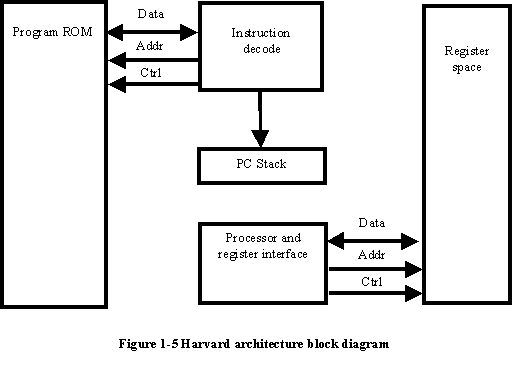
\includegraphics[width=0.5\linewidth]{microcontrollore/assets/Harvard.png}
    \caption{Struttura interna del microcontrollore}
\end{figure}
Questa architettura, unita ad un doppio bus asincrono, permette di eseguire più operazioni in parallelo, aumentando la velocità di esecuzione. Un esempio del perchè questa architettura sia più veloce deriva dal fatto che in un singolo colpo di clock, il microcontrollore sia in grado di leggere l'istruzione e interagire con il dato da modificare.\\

\subsubsection{Memoria}
All'interno del microcontrollore esistono 3 tipi di memoria:
\begin{itemize}
    \item Flash: Una memoria non volatile che sacrifica la velocità di scrittura per aumentare la capacità di lettura. Nei microcontrollori è usata per salvare i programmi.
    \item RAM: Una memoria volatile con lo scopo di salvare i dati della singola esecuzione del programma. Per stare al passo con la CPU serve velocità di lettura e scrittura
    \item ROM: Una memoria non volatile di sola lettura. Viene scritta dai produttori e contiene informazioni fondamentali per il corretto funzionamento del microcontrollore, oltre alla definizione di registri e celle di memoria speciale.
\end{itemize}
Ogni memoria è divisa in celle, ognuna delle dimensioni di un byte e caratterizzata da un indirizzo unico. Per salvare dati più grandi di un byte, si usano più celle contigue, così che sapendo dimensione del dato e indirizzo di partenza, si possa trovare univocamente il dato.\\
La memoria è connessa alla CPU con dei BUS dedicati.

Per quanto riguarda la RAM, oltre ad essere divisa in celle, i produttori della scheda dividono la memoria dedicata alle periferiche in registri. Dandogli dei ruoli specifici all'interno della CPU. Questa divisione permette di avere un modo più semplice di collegare le celle di memoria al loro significato e permette alla CPU di lavorare in maniera più efficiente sulle celle di memoria a utilizzi speciali.

Nella memoria Flash, invece, i programmi sono salvati in pile di celle di memoria, ognuna con un codice operativo che, letto dalla CPU, si trasforma in un'istruzione. L'istruzione in questione non ha accesso solo alla RAM in cui sono contenuti i dati di esecuzione ma anche alla memoria flash stessa; questo permette alla CPU di saltare istruzioni o di ripeterle nel caso in cui sia richiesto.



\subsection{Periferiche}

Il microcontrollore è dotato di diverse periferiche e funzionalità ma noi siamo andati a guardare solo quelle interessanti allo scopo di trattare dati analogici e digitali. Queste funzionalità sono:
\begin{itemize}
    \item Timer
    \item Universal Synchronous Asynchronous Receiver Transmitter (USART)
    \item Analog Digital Converter (ADC)
    \item Direct Memory Access (DMA)
    \item Digital Analog Converter (DAC)
    \item Comparatore
\end{itemize}
In particolare, USART è utile per trasmettere dati al computer con la seriale, l'ADC per leggere dati analogici, il timer per triggerare il tempo tra una misura e l'altra in modo da avere misure equidistanti, il DMA per trasferire i dati tra la memoria e le periferiche senza l'intervento della CPU e il DAC e il comparatore per creare dei meccanismi di trigger hardware.



\pagebreak

\subsection{Programmazione}
Per programmare sul microcontrollore è stato usato il programma STM32CubeIDE, un IDE fornito dalla STMicroelectronics. Il linguaggio di programmazione usato è C99. All'interno dell'IDE sono inserite delle librerie che permettono di interfacciarsi con le periferiche del microcontrollore, le quali contengono gli indirizzi dei registri e le maschere per collegare ogni bit dei registri al funzionamento sulla periferica.\\

I registri prendono il nome dalla periferica che controllano e ogni registro è diviso in sottoregistri a cui si può accedere usando i puntatori.

Per modificare i registri è consigliato usare maaschere, quindi dei numeri binari che, se applicate delle operazioni di AND e OR permettono di andare a modificare solo determinati bit.

\subsubsection{Struttura del programma}
Il programma si divide in diversi file:
\begin{itemize}
    \item \textbf{main.c}: Il file principale del programma, contiene la funzione main() e le funzioni di inizializzazione delle periferiche. Il compilatore lancia il programma a partire da questo file.
    \item \textbf{stm32h7xx$\_$it.c}: Il file contenente tutti gli interrupt abilitati. Ogni interrupt è una funzione diversa che non comunica direttamente con il resto.
    \item \textbf{Librerie create dall'utente}: File contenenti le funzioni create dall'utente per interfacciarsi con le periferiche.
\end{itemize}

Questi sono solo alcuni dei file presenti nel progetto, ma sono quelli che effettivamente modificati dall'utente.

\subsubsection{ Interrupt }
Tutte le implementazioni delle funzionalità sono state fatte usando i relativi Interrupt. Un interrupt è un segnale che viene inviato alla CPU per interrompere l'istruzione in corso e dare priorità ad un'altra istruzione. Questo meccanismo permette di rimanere in attesa di un evento senza dover per forza limitarsi a controllare ciclicamente se è avvenuto.\\
Così facendo si è in grado di fare più cose contemporaneamente e di ottimizzare la velocità di esecuzione del programma.\\

Ogni periferica ha uno o più interrupt dedicati che vengono attivati con eventi diversi. In particolare:
\begin{itemize}
    \item \textbf{USART}: Ha un interrupt dedicato per la ricezione e uno per la trasmissione, che vengono chiamati quando il buffer in ricezione è pieno o quando il buffer in trasmissione è vuoto.
    \item \textbf{ADC}: Ha un interrupt dedicato per la fine della conversione, che viene chiamati quando il valore analogico è stato convertito in digitale.
    \item \textbf{DMA}: Ha un interrupt dedicato per la fine del trasferimento, che viene chiamato quando il trasferimento di dati è finito.
    \item \textbf{Timer}: Ha un interrupt dedicato per la fine del conteggio, che viene chiamato quando il timer ha finito di contare.
\end{itemize}

Per ogni interrupt, esiste una funzione creata ad hoc che possiamo riempire con il codice che vogliamo e che possiamo decidere se attivare o disattivare a piacimento.



\pagebreak
\section{Universal Synchronous Asynchronous Receiver Transmitter (USART)}
La prima periferica usata è stata la USART. Usart ci permette di comunicare con il PC attraverso la Seriale.
\\

\subsection{Funzionamento}
Seppur la periferica permetta il trasferimento sicrono dei dati, noi la useremo come USART, quindi una versione precedente.\\

Questa periferica per funzionare ha bisogno di un collegamento diretto con il dispositivo a cui comunicare, questo collegamento nel nostro cavo consiste in 3 cavi: TX, RX e GND.\\


\noindent
\begin{minipage}[c]{0.54\linewidth}
    \begin{itemize}
        \item TX: Trasmettitore, invia i dati al PC
        \item RX: Ricevitore, riceve i dati dal PC
        \item GND: Collegamento a terra, serve per chiudere il circuito e tarare entrambi i dispositivi allo stesso 0
    \end{itemize}
\end{minipage}
\hfill
\begin{minipage}[t]{0.4\linewidth}

    \centering
    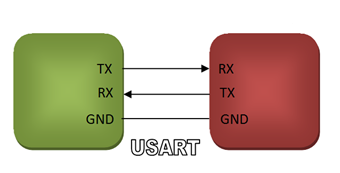
\includegraphics[width=0.7\linewidth]{microcontrollore/assets/USART.png}
    \label{fig:USART}
    \captionof{figure}{Collegamento tra microcontrollore e PC}
\end{minipage}

I dati sono mandati sottoforma di impulsi elettrici. Dato che i due dispositivi sono collegati con un singolo cavo, i dati sono inviati in ordine e, l'unica cosa di cui i due dispositivi hanno bisogno è la velocità di trasmissione, che deve essere uguale tra i 2 per assicurare la giusta lettura.\\
La velocità di trasmissione è misurata in baud, ovvero il numero di bit trasmessi in un secondo e per questo si chiama Baud Rate. Di base è a 9600 baud, ma a seconda delle necessità può essere alzata fino al limite strumentale.\\

Per evitare problemi di lettura, il ricevitore overcampiona i dati per poi farne una media. Così facendo, il rumore dovuto a cavi troppo lunghi o a interferenze elettromagnetiche viene minimizzato.\\


\subsection{Programmazione}
Usart, nel nostro caso, è stato usare nel seguente modo: Inizialmente abbiamo spedito un carattere specifico dal pc al microcontrollore, questo carattere l'abbiamo usato come trigger per far partire la lettura dei dati, finita la lettura dei dati abbiamo trasmesso tutti i dati al computer.\\

\noindent
\begin{minted}[bgcolor = coding, linenos]{C}
void ESPE_USART_char_start(void){

    if ( USART3 ->ISR & USART_ISR_RXNE_RXFNE){ // Se il buffer è pieno
        if ( USART3 -> RDR == char_trigger){ // Se il carattere è uguale al trigger
            flag_Trigger_EN = 1;

        }
    }
}
\end{minted}
\label{code:USART_start}

Nel codice {\hypersetup{linkcolor=black}\ref{code:USART_start}}, andiamo ad usare 2 registri di USART: ISR e RDR. Il primo, l'Interrupt Status Register, contiene flag per controllare lo status di USART, mentre il secondo, il Receive Data Register, contiene il dato ricevuto.\\

\noindent
\begin{minted}[bgcolor = coding, linenos]{C}
#define len_vec 100
uint_8 vec_dati[len_vec];
uint_8 len = sizeof(uint_8)/sizeof(char)*len_vec;
char *str = vec_dati;
uint_8 indice = 0;


void ESPE_USART_send_data(void){
    if( USART3 ->ISR & USART_ISR_TC){ // Se il buffer è vuoto
		if (indice < len){
			USART3->TDR = *(str+indice); // Invia il dato
			indice++;
		}else{
			if(indice == len){
				USART3 -> TDR = '\r'; // Invia il carattere di fine riga
				indice = 0;
			}
		}
	}
}
\end{minted}
\label{code:USART_send}

In questo codice, invece andiamo a usare il registro TDR, il Transmission Data Register, per mandare i dati al PC, ma, dato che i dati sono messi in un vettore di uint8 e il TDR ha le dimensioni di un char, il numero di byte da inviare non corrisponde alla dimensione del vettore. Questa discrepanza è risolta dalla variabile *str che è una variabile puntatore di tipo char puntata all'inizio del vettore.\\


Oltre a queste funzioni è necessario definire un'altra funzione ausiliaria con la quale si passa dalla lettura dei dati al loro invio.\\

\noindent
\begin{minted}[bgcolor = coding, linenos]{C}
void ESPE_USART_invert_mode(void){
    if(USART3 -> CR1 & USART_CR1_RXNEIE){
        USART3 -> CR1 &= ~USART_CR1_RXNEIE;
        USART3 -> CR1 |= USART_CR1_TCIE;
    }else if(USART3 -> CR1 & USART_CR1_TCIE){
        USART3 -> CR1 |= USART_CR1_RXNEIE;
        USART3 -> CR1 &= ~USART_CR1_TCIE;
    }
}
\end{minted}

Questa funzione cambia il metodo di trigger dell'interrupt di USART, così facendo si evitano problemi con interrupt in lettura mentre l'invio è in corso o viceversa.\\





\pagebreak
\section{Analog Digital Converter (ADC)}
L'ADC è una periferica che permette di convertire un segnale analogico in un segnale digitale. 

\subsection{Funzionamento}
Per convertire valori analogici in digitale esistono diversi metodi, il microcontrollore usato usa il metodo di conversione ad approssimazioni successive.\\

Seppur questo metodo non permette di avere i dati convertiti istantaneamente come può essere un Flash ADC, permette di avere una maggiore precisione e di avere un errore minore.\\

\begin{wrapfigure}{l}{0.7\linewidth}
    % \centering
    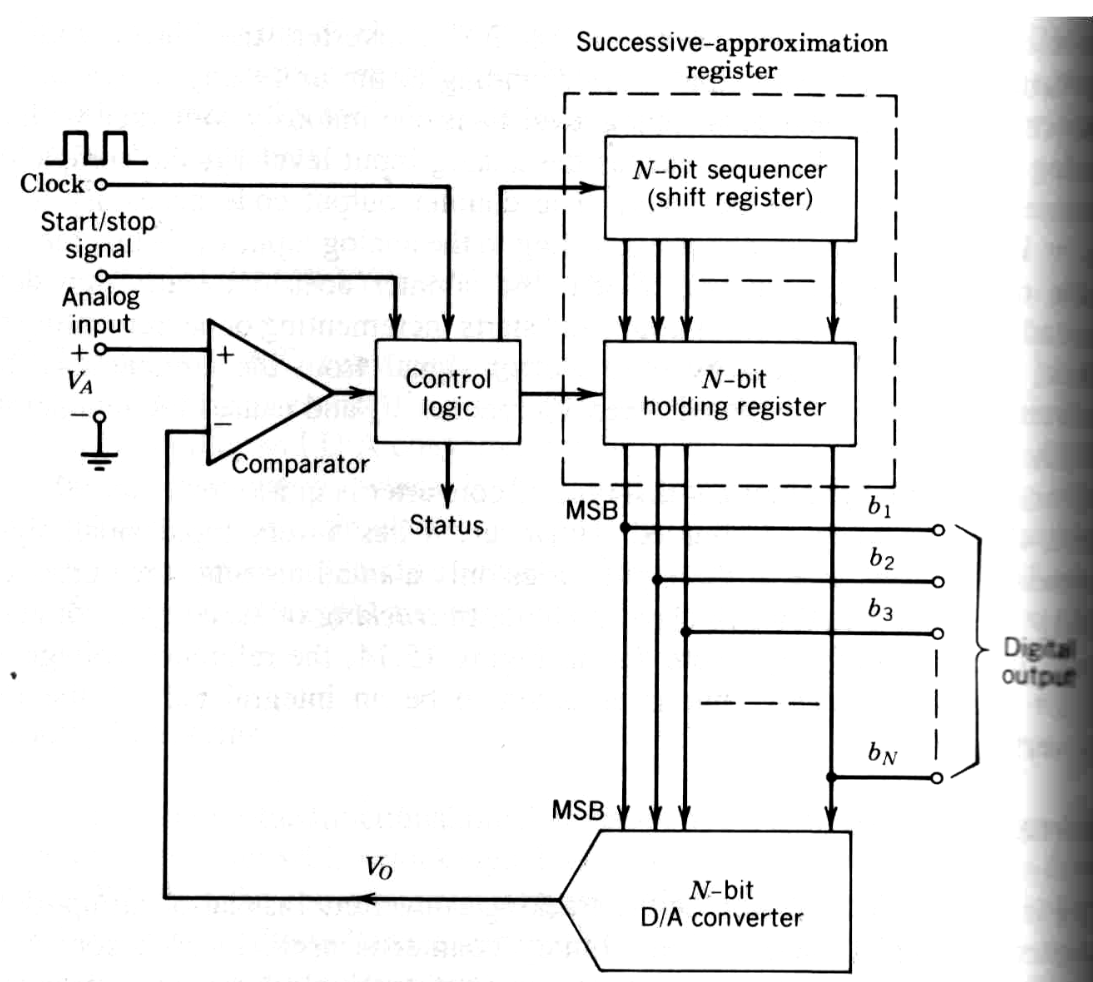
\includegraphics[width=0.8\linewidth]{microcontrollore/assets/ADC.png}
    \label{fig:ADC}
    \captionof{figure}{Schema di funzionamento dell'ADC}
\end{wrapfigure}

L'ADC ad approssimazioni successive per funzionare sfrutta un comparatore e un metodo di ricerca binaria. Attraverso una coversione Digitale-Analogica, il microcontrollore invia un segnale analogico al comparatore, il quale ritornerà un segnale positivo se il segnale inviato è maggiore di quello ricevuto, altrimenti ritornerà nullo.\\

Così facendo, il microcontrollore può ricavare con precisione e con poche iterazioni del metodo la rappresentazione binaria migliore per il valore analogico.\\

Altri aspetti positivi di questo metodo sono la presenza di un singolo compartore, il quale permette di diminuire notevolmente l'errore nella misura e la presenza di registri per la ricerca binaria, i quali rendono il processo più veloce di altri metodi.\\

\subsection{Programmazione}
Parte importante della programmazione con l'ADC è la calibrazione dell'apparato. Infatti, prima dell'utilizzo

\noindent
\begin{minted}[bgcolor = coding, linenos]{C}
    void ESPE_ADC_init(void){

	// azzeriamo per evitare casini di configurazione
	ADC3 -> SQR1 = 0;

	// ogni numero è collegato ad un pin a sèstante
	ADC3->SQR1 |= 0 <<ADC_SQR1_L_Pos;// ti dice quante misure deve prendere (n+1)
	ADC3->SQR1 |= 0 << ADC_SQR1_SQ1_Pos; // ti dice qual è la prima misura da fare

	ADC3->PCSEL |= ADC_PCSEL_PCSEL_0;//segna quali sono i canali in lettura per
                                        //velocità massima

	ADC3 -> CR &= ~ADC_CR_DEEPPWD_Pos;//Deep power down state
                                        //(se attivo non overclocka)
	ADC3 -> CR |= 1 << ADC_CR_ADVREGEN_Pos;//Voltage regulator activated

	ADC3 -> CR &= ~ADC_CR_ADCALDIF_Pos;//seleziona modalità differenziata
                                            //di calibrazione (a 0)
	ADC3 -> CR |= 1<< ADC_CR_ADCALLIN_Pos;//seleziona la modalità lineare
                                            //di calibrazione (a 1)
	ADC3 -> CR &= ~ADC_CR_ADEN_Pos;//Controlliamo che l'ADC non sia acceso e che
                                            //il bit sia stato resettato
	ADC3 -> CR |= 1<< ADC_CR_ADCAL_Pos;// Inizia la calibrazione

	while( ADC3->CR & ADC_CR_ADCAL ){							
            //Aspetti che la calibrazione sia finita, il bit viene cambiato dall'hardware
	}

	ADC3->ISR &= ~ADC_ISR_ADRDY_Pos;//Controlli che il bit per l'inizio della
                                        //presa dati sia a 0
	ADC3->CR |= 1<<ADC_CR_ADEN_Pos;//Attiviamo l'ADC (non la presa dati)
	while( !(ADC3->ISR & ADC_ISR_ADRDY)){						
            //Aspettiamo che sia setuppato correttamente
	}

	ADC3 -> IER |= ADC_IER_EOCIE;//Attiviamo l'interrupt

	ADC3 -> SMPR1 |= 0<<ADC_SMPR1_SMP0_Pos;
        //Possiamo aggiungere un ritardo di (n = 0) cicli prima della lettura

    }
\end{minted}
\label{code:ADC_init}

Oltre a impostare le misure da fare e il numero di misure che ogni ADC deve fare su ogni pin, all'interno della funzione è contenuto il processo di calibrazione dell'ADC. La calibrazione è fatta automaticamente dal microcontrollore usando dei valori di riferimento ma questo processo occupa tempo e, se non si aspettasse la fine della calibrazione per prendere la misura si avrebbero valori errati. Quindi c'è bisogno di un ciclo \textit{while()} per aspettare la fine della calibrazione.\\

La calibrazione è fatta accedendo a 2 Registri in particolare: il registro CR e il registro ISR. Il primo contiene i bit per la calibrazione e l'attivazione dell'ADC, mentre il secondo contiene i bit per controllare lo stato dell'ADC.\\

Una volta finita la calibrazione,  scrivendo
\noindent

\begin{minted}[bgcolor = coding]{C}
    ADC3-> CR |= ADC_CR_ADSTART
\end{minted}
l'ADC inizia a prendere le misure.\\
Per leggere i dati, invece, si può inserire nell'interrupt una funzione dedicata del tipo:

\noindent
\begin{minted}[bgcolor=coding , linenos]{C}

    #define len_vec 100
    uint_16 vec[len_vec];
    uint_8 counter_ADC = 0;
    uint_8 conversion_flag = 0;

    void ESPE_ADC_data(void){
        if( counter_ADC < len_vec){
            vec[counter_ADC] = ADC3->DR;
            counter_ADC++;
        }else{
            conversion_flag = 1;
            ADC3-> CR &= ~ADC_CR_ADSTART;
        }
    }

\end{minted}
\label{code:ADC_data}

In questo codice, il registro DR, il Data Register, contiene il valore misurato dall'ADC in Volt. Se il valore che si vuole non è in volt, è necessario fare una conversione. La conversione dipende da fattori come la tensione di riferimento dell'apparecchio che fa la misura e il valore massimo misurabile dall'ADC.\\

L'ultima riga, invece è necessaria per fermare l'ADC una volta che ha finito di prendere le misure.\\

\pagebreak
\section{Direct Memory Access (DMA)}
Usando ADC e USART per fare misure e trasferire dati, una delle più grandi limitazioni in velocità è il tempo di trasferimento dei dati dalla periferica al microcontrollore. Questo tempo è dovuto al fatto che la CPU deve leggere i dati dalla periferica e salvarli in memoria.\\

\subsection{Funzionamento}

Il processo per trasferire dati dalla periferica alla memoria presume che il dato, prima di essere salvato nella memoria RAM, sia salvato nella memoria interna alla CPU in modo che la CPU ci possa lavorare. \\
Questo passaggio si può rimuovere usando il DMA.

\begin{figure}[h]
    \centering
    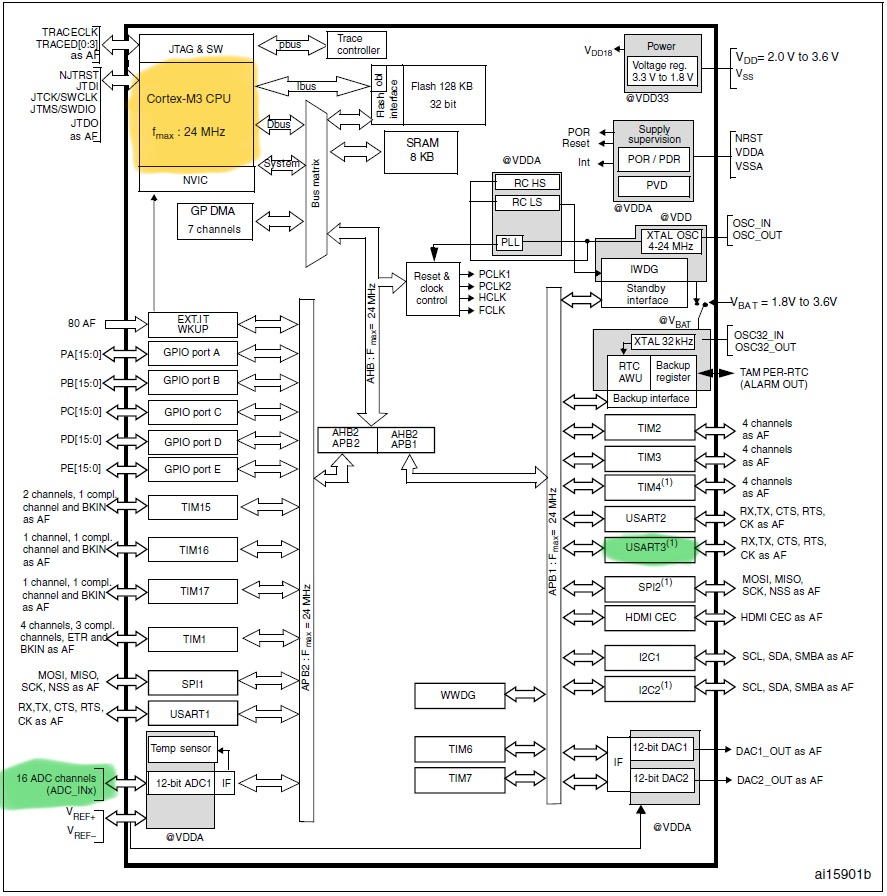
\includegraphics[width=0.8\linewidth]{microcontrollore/assets/Cortex_structure.jpg}
    \caption{Struttura interna del microcontrollore}
    \label{fig:Cortex}
\end{figure}

Una volta configurato, il DMA permette di evitare il carico computazionale della CPU per il trasferimento dei dati dando l'accesso diretto alla periferica di accedere alla memoria.
Così facendo, oltre alla CPU più libera, i dati saranno salvati direttamente dalle periferiche nella memoria nella maniera più veloce possibile.\\

\subsection{Programmazione}
Dato che il protocollo del DMA ti permette di salvare i dati in autonomia, la parte di programmazione consiste solo nel configurare correttamente il DMA.\\



Dato che può essere molto complesso, parte della configurazione è stata fatta con il code generator di STM32CubeIDE e consiste nel collegare uno \textit{stream} del DMA alla periferica che si vuole usare e dargli la dimensione del dato e in che tipo di memoria si vuole salvare.\\

\begin{wrapfigure}{r}{0.4\linewidth}
    \centering
    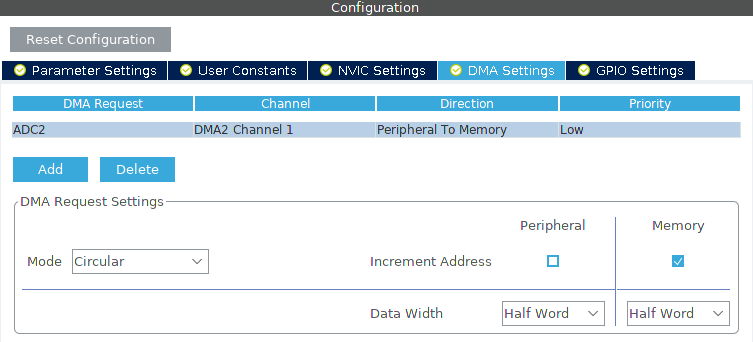
\includegraphics[width=\linewidth]{microcontrollore/assets/dma_configuration.png}
    \caption{Configurazione del DMA}
    \label{fig:DMA}
\end{wrapfigure}

Una volta configurato su STM32CubeMX, c'è bisogno di configurare specificatamente il DMA per la periferica che si vuole usare e aggiungere alla periferica l'istruzione che permette di essere collegata al DMA.\\

In generale, questo tipo di configurazione può essere riassunta in 4 righe di codice. Usiamo come esempio il DMA per l'ADC:

\begin{minted}[bgcolor = coding, linenos]{C}
    DMA1_Stream0 -> PAR = (uint32_t) &ADC3->DR; //Collegare il DMA al registro
                                                //che contiene il dato
    DMA1_Stream0 -> M0AR = (uint32_t) &vec_dati; //Dare al DMA l'indirizzo della memoria
                                                //in cui salvare il dato
    DMA1_Stream0 -> NDTR = len; // Dimensione del dato
    ADC3 -> CFGR |=(3<<ADC_CFGR_DMNGT_Pos); // Configura l'ADC per usare il DMA
\end{minted}

e poi si attiva il DMA con la funzione:

\begin{minted}[bgcolor = coding, linenos]{C}
    DMA1_Stream0->CR |= DMA_SxCR_EN // Attiva il DMA
\end{minted}

\begin{flushleft}

    \colorbox{notebox}{
    \begin{minipage}[]{\textwidth}
        Notiamo come, anche se il DMA è attivo, ciò non va a modificare il funzionamento degli interrupt. Anche se il DMA controlla il flusso dei dati, noi possiamo comunque accedere a qualsiasi dato (misurato o trasmesso) in qualsiasi momento.
    \end{minipage}
    }
\end{flushleft}

\pagebreak
\section{Timer}
Parte fondamentale per il funzionamento del microcontrollore è il Timer. In particolare, il timer è fondamentale per scandire il rateo delle operazioni della CPU e per dare un tempo di esecuzione alle periferiche.\\

Nel microcontrollore che abbiamo usato non c'è un singolo timer e ognuno ha caratteristiche, precisione e funzionalità diverse. 
Per i nostri scopi, noi abbiamo interagito con il Timer 6 che è un timer PLL

\subsection{Funzionamento}
I clock PLL sono dei clock che sfruttano un clock di riferimento, nel nostro caso di quarzo, per generare un clock a frequenze più alte. Questo processo avviene attraverso un Voltage Control Oscillator il quale è in grado di generare onde quadre a frequenze molto alte e un
Filtro passa Basso che fa da filtro per le armoniche generate dal VCO.\\

\begin{figure}[h]
    \centering
    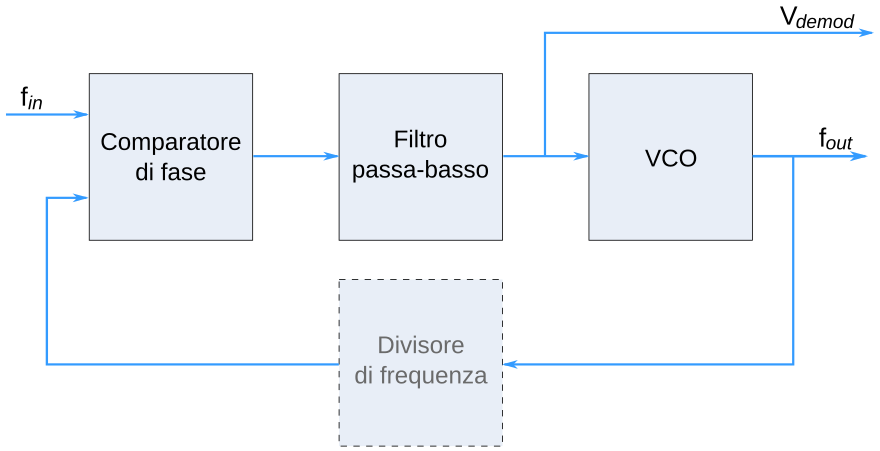
\includegraphics[width=0.7\linewidth]{microcontrollore/assets/PLL1_it.png}
    \caption{Schema di funzionamento del Timer}
    \label{fig:Timer}
\end{figure}

Questi 2 componenti, collegati ad un comparatore e al cristallo di riferimento riescono a generare onde quadre ad un ritmo costante usando il quarzo, molto stabile, come riferimento per non perdere la periodicità.\\
A questo processo si aggiungono altri componenti come il prescaler e il contatore che permettono di avere un controllo più preciso sulla frequenza del clock generato.\\

Per avere la massima velocità di esecuzione del programma, vanno modificate le frequenze dei clock. Così facendo, si possono velocizzare i processi più lenti a discapito di altri e di un maggior consumo di energia.\\

\subsection{Programmazione}
Per configurare il Timer 6, abbiamo usato STM32CubeMX. Questo programma permette di configurare ogni singolo timer a piacere, a patto di non uscire dai limiti del microcontrollore. Questo processo si fa attraverso un'interfaccia grafica dedicata

\begin{figure}
    \centering
    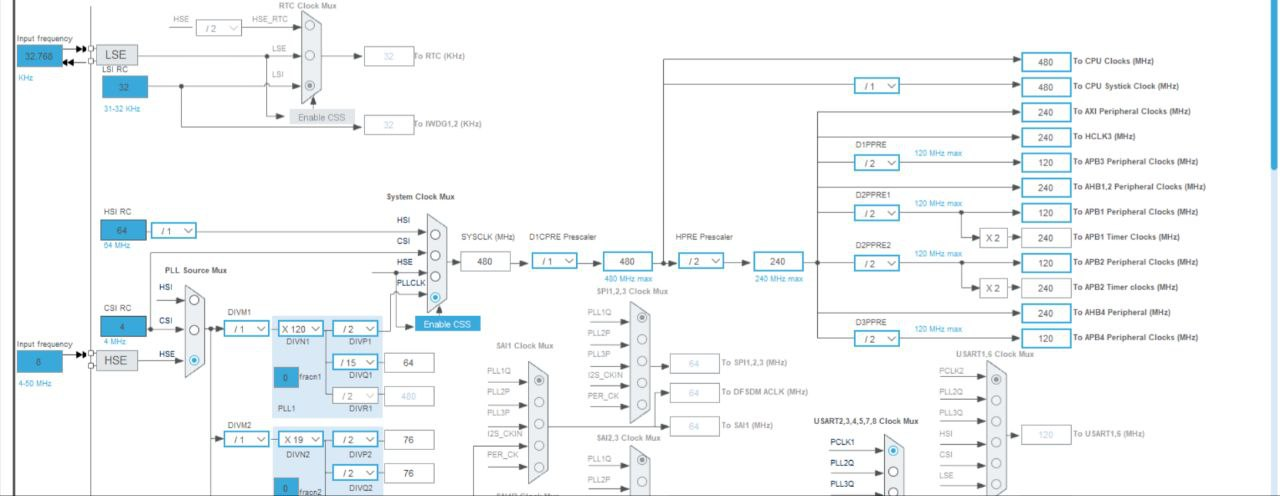
\includegraphics[width=0.7\linewidth]{microcontrollore/assets/clock_config.jpg}
    \caption{Configurazione del Timer}
    \label{fig:Timer}
\end{figure}
 
Una volta configurato, si può passare all'inizializzazione del Timer.

\begin{minted}[bgcolor=coding , linenos]{C}
    void ESPE_TIM6_init(void){
        TIM6->CNT = 0; //Resetta il contatore
        TIM6->ARR = 10;//Setta il valore di auto reload
        TIM6->PSC = 24;//Setta il prescaler
    }
\end{minted}

Così facendo si può ulteriormente modificare la frequenza del timer e quindi la velocità delle periferiche ad essere collegate.\\
Per attivare il timer, si usa la funzione:
\begin{minted}[bgcolor=coding , linenos]{C}
    TIM6->CR1 |= TIM_CR1_CEN;
\end{minted}

Nel caso ce ne sia necessità il timer ha anche un interrupt che viene chiamato quando il contatore arriva al valore di auto reload, ma l'utilizzo del timer è stato quello di collegarlo all'ADC per far sì di avere misure equamente distanziate nel tempo, cosa non scontata a causa del metodo di conversione dell'ADC.\\

\pagebreak
\section{Digital Analog Converter (DAC) e Comparatore}
Il DAC e il Comparatore, seppur 2 periferiche diverse, sono trattate insieme in quanto sono usate come trigger: il DAC per generare un segnale analogico e il comparatore per confrontare il segnale generato con un segnale di riferimento, così facendo si può avere un meccanismo di Trigger molto preciso e veloce.\\

\subsection{Funzionamento DAC}

Il DAC del microcontrollore è una periferica a 12 bit che permette di generare un segnale analogico a partire da un segnale digitale.\\ 
Una grande problematica del DAC è la gestione dell'errore. Infatti, se si vuole generare un segnale analogico ad un determinato voltaggio a partire da un numero binario, a prescindere dalla struttura, ci sarà sempre un errore dovuto alla lunghezza del numero binario. A questo errore si aggiungono tutti gli errori strumentali delle componenti del DAC.\\

Per questo motivo, la struttura del DAC è stata progettata in modo da minimizzare l'errore. Questa struttura è detta \textit{R-2R} e consiste in una rete di resistenze dal valore di $R$ e $2R$.

\begin{figure}[h]
    \centering
    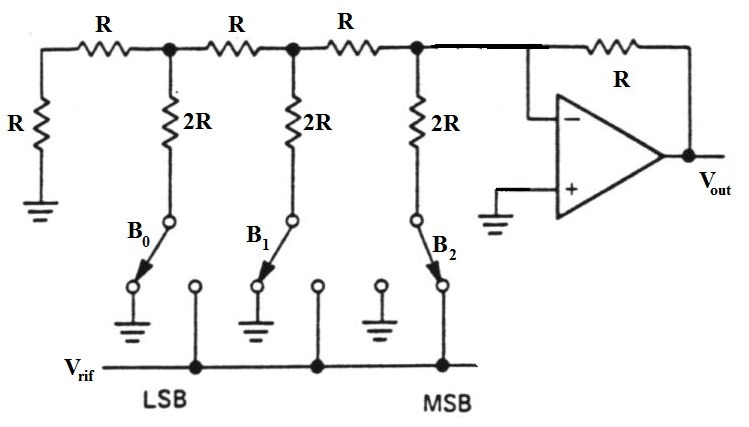
\includegraphics[width=0.7\linewidth]{microcontrollore/assets/DACr2r.jpg}
    \caption{Struttura interna del DAC}
    \label{fig:DAC}
\end{figure}

La struttura è molto semplice: se il bit è 1, il circuito si chiude e il voltaggio in uscita è $V_{ref}$, se il bit è 0, il circuito si apre e il voltaggio in uscita è 0. La configurazione delle Resistenze permette di dimezzare il voltaggio in uscita ad ogni iterazione dello schema. E, dato che alla fine c'è un amplificatore operazionale, il voltaggio in uscita sarà la somma dei voltaggi generati da ogni bit, moltiplicato per un fattore dell'Amplificatore.\\

Così facendo, usando solo 2 tipi di resistenza, un amplificatore operazionale e dei transistore come interruttori, siamo in grado di creare un segnale analogico.\\
\pagebreak
\subsection{Funzionamento Comparatore}
Il Comparatore non è altro che un amplificatore operazionale con un'uscita che non può essere Negativa. Questo significa che, se il voltaggio in ingresso è maggiore di un voltaggio di riferimento, l'uscita sarà alta, altrimenti sarà bassa.\\

\begin{wrapfigure}{r}{0.4\linewidth}
    \centering
    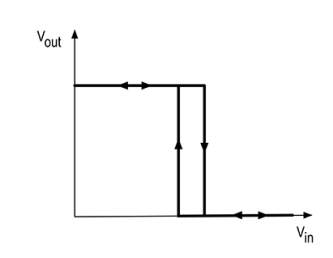
\includegraphics[width=\linewidth]{microcontrollore/assets/Hysteresis.png}
    \caption{Grafico Voltaggio Amplificatore con Isteresi}
    \label{fig:Comparatore}
\end{wrapfigure}
Un comportamento particolare del comparatore è l'isteresi. L'isteresi è un fenomeno che si verifica quando il segnale in ingresso è vicino al voltaggio di riferimento. In questo caso, l'uscita del comparatore non è stabile e può oscillare tra alto e basso. Per evitare questo fenomeno, si può aggiungere un isteresi al comparatore.\\
L'isteresi si aggiunge mettendo un partitore di tensione in retroazione positiva. Così facendo ci sarà una differenza di voltaggio tra quando il comparatore sale e quando scende.\\

Questo comportamento ci permetterà di usare il comparatore non solo come singolo trigger ma come doppio trigger.\\

\subsection{Programmazione}
La programmazione del DAC e del Comparatore si fa quasi totalmente da STM32CubeMX. La configurazione consiste nel collegare il DAC al comparatore, selezionre il valore di isteresi del Comparatore. Una volta configurato, nel codice basta aggiungere la funzione che permette di attivare il DAC e il Comparatore.\\

\begin{minted}[bgcolor=coding , linenos]{C}
    COMP2->CFGR |= COMP_CFGRx_EN; // Attiva il Comparatore
    DAC1 -> DHR12R1 = 1000;	// soglia di trigger
	DAC1 -> SWTRIGR |= DAC_SWTRIGR_SWTRIG1; // Abilita il software trigger
	DAC1 -> CR |= DAC_CR_EN1; // Attiva il DAC
\end{minted}

E, per andare a controllare lo stato del comparatore, si può usare la funzione:

\begin{minted}[bgcolor=coding , linenos]{C}
if( COMP12 -> SR & COMP_SR_C2VAL){ // Se il comparatore è attivo
    //Fai qualcosa
}
\end{minted}